\documentclass[9pt]{beamer}

\usetheme[progressbar=frametitle,block=fill,background=light]{metropolis}
\usefonttheme{serif}

\usepackage{appendixnumberbeamer}

\usepackage{booktabs}
\usepackage[scale=2]{ccicons}


\usepackage{pgfplots}
\usepgfplotslibrary{dateplot}
\usepackage{pgfplotsthemetol}
\usepackage{amsmath,amssymb,amsthm,amsfonts,amstext}
\usepackage{bbm}
\usepackage{array}
\usepackage{multimedia}
\usepackage{media9}

\usepackage{xspace}
\usepackage{emoji}

\usepackage{import}
\import{}{Packages/custom_macros.tex}

\makeatletter
\setlength{\metropolis@titleseparator@linewidth}{2pt}
\setlength{\metropolis@progressonsectionpage@linewidth}{2pt}
\setlength{\metropolis@progressinheadfoot@linewidth}{2pt}
\makeatother

\newcommand{\themename}{\textbf{\textsc{metropolis}}\xspace}
\renewcommand{\emph}{\alert}

\title{Group theory, Topology and Spin-$1/2$ Particles}
\subtitle{From Dirac's belt to fermions}
% \date{\today}
\date{}
\author{Louan Mol}
\institute{Unversité Libre de Bruxelles\\[2cm]{\small Brussels Summer School of Mathematics 2022}}
% \titlegraphic{\hfill\includegraphics[height=1.5cm]{logo.pdf}}

\begin{document}

\maketitle

\nocite{*}

\begin{frame}{Table of contents}
    \setbeamertemplate{section in toc}[sections numbered]
    \tableofcontents%[hideallsubsections]
\end{frame}

\section{Dirac's belt trick and the rotation group}

\begin{frame}{Dirac's belt trick}
    
    You need:
    \begin{itemize}
        \item a belt (not necessarily Dirac's)
        \item a heavy book
    \end{itemize}
    Rules:
    \begin{enumerate}
        \item you can only move the end of the belt
        \item you cannot twist or rotate it
    \end{enumerate}
    \textbf{Goal:} untwist a $2\pi$-twist.\\[0.5cm]
    $\Rightarrow$ it tuns out to be \emph{impossible} ! One turn negates the twist: $2\pi\to-2\pi$. \\[0.5cm]

    Therefore, possible for a $4\pi$ twist ...\\ \hspace{7cm} Why is that ?

\end{frame}

\begin{frame}{Space of rotations: $\SO(3)$ as a group}
      
    Rotations in $3$-dimensional space: matrices that acts on $\R^3$ s.t. 
    \begin{enumerate}
        \item preserve the \emph{scalar product}: $O^TO=\mathbbm{1}$ ($\Leftrightarrow$ $O$ is orthogonal)
        \item preserve the \emph{orientation}: $\det O=1$
    \end{enumerate}

    \begin{block}{Special othogonal group}
        $\SO(3)$ is the set of $3\times 3$ real matrices such that $O^TO=\mathbbm{1}$ and $\det O=1$.
    \end{block}
    Three ``fundamental'' rotations:
    \begin{equation*}
      {\tiny
      x:
      \begin{bmatrix}
          1 & 0 & 0 \\
          0 & \cos\theta & -\sin\theta \\
          0 & \sin\theta & \cos\theta
      \end{bmatrix}\qquad
      y:
      \begin{bmatrix}
          \cos\theta & 0 & -\sin\theta \\
          0 & 1 & 0 \\
          \sin\theta & 0 & \cos\theta
      \end{bmatrix}\qquad
      z:
      \begin{bmatrix}
          \cos\theta & -\sin\theta & 0 \\
          \sin\theta & \cos\theta & 0 \\
          0 & 0 & 1
      \end{bmatrix}}
    \end{equation*}

    $\Rightarrow$ It forms a \emph{group}.
    
\end{frame}

\begin{frame}{Space of rotations: $\SO(3)$ as a topological space}
    Fundamental data that describes a rotation:
    \begin{itemize}
        \item an \emph{axis} of rotation, i.e. a  unit vector $\overrightarrow{n}$ \hspace{1.07cm}\textcolor{blue}{$\to$ 2 parameters}
        \item an \emph{angle} of rotation $\theta\in[-\pi,\pi]$ (with $-\pi\sim\pi$) \textcolor{blue}{$\to$ 1 parameter}
    \end{itemize}
    The space of rotations can then alternately be defined as a \textbf{$\boldsymbol{3}$-sphere of radius $\boldsymbol{\pi}$ and its antipodal points identified}:
    

    \begin{columns}[T,onlytextwidth]
        \column{0.5\textwidth}

            \vspace{0.5cm}
            \begin{equation*}
              \boxed{\SO(3)\cong B^3(\pi)/\sim}
            \end{equation*}
            and for each point:
            \begin{align*}
                \text{direction} &\leftrightarrow \text{axis}\\
                \text{norm} &\leftrightarrow \text{angle}
            \end{align*}
            $\Rightarrow$ It forms a \emph{topological space}.
  
        \column{0.5\textwidth}
  
            \begin{figure}
                \centering
                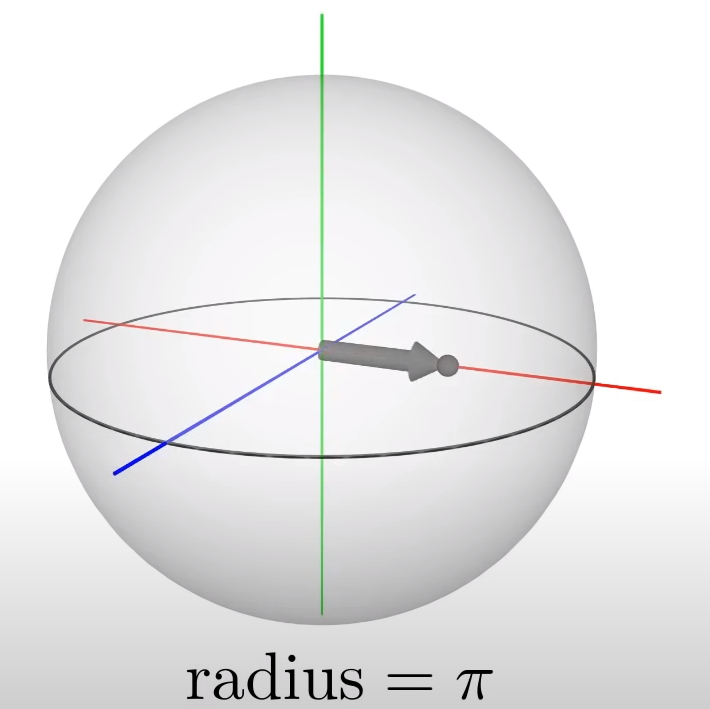
\includegraphics[scale=0.16]{Pictures/SO3sphere.png}
            \end{figure}
  
    \end{columns}

    (group $+$ topological space $=$ Lie group)
    
\end{frame}

\begin{frame}{Back to the belt}

    Mathematical description of the belt ?\\[0.3cm]
    \quad $\triangleright$ a belt is a strip, which is just a \emph{path} $+$ an \emph{orientation}.\\[0.2cm]
    \quad $\triangleright$ given axis on the middle line along the belt, each set of axis \\ \hspace{0.5cm} is related by a rotation \\[0.2cm]
    \quad $\triangleright$ a belt configuration is equivalent to a continuous set of axis and \\ \hspace{0.5cm} therefore to a continuous set of translations, i.e. a \emph{path in $\SO(3)$}
    \begin{figure}
        \centering
        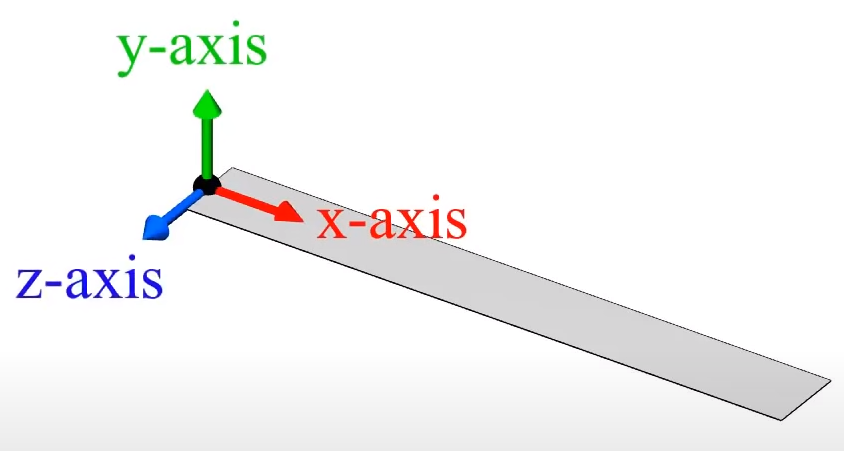
\includegraphics[scale=0.12]{Pictures/beltaxis.png}
    \end{figure}
    There is a bijection:
    \begin{equation*}
        \boxed{\text{belt configuration} \Leftrightarrow \text{path in $\SO(3)$}}
    \end{equation*}
    This gives us a new language to analyze the problem !

\end{frame}

\begin{frame}{Dictionary}
    \makebox[315pt][r]{
    \begin{tabular}{cccc}
        \textbf{\underline{trivial rotation}} & \textbf{\underline{$2\pi$ \textcolor{red}{$x$}-rotation}} & \textbf{\underline{$2\pi$ \textcolor{green}{$y$}-rotation}} & \textbf{\underline{$2\pi$ \textcolor{blue}{$z$}-rotation}}\\
        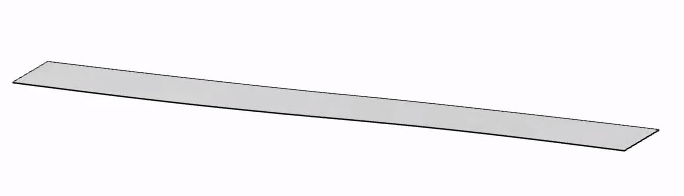
\includegraphics[scale=0.12]{Pictures/flatbelt.png} & 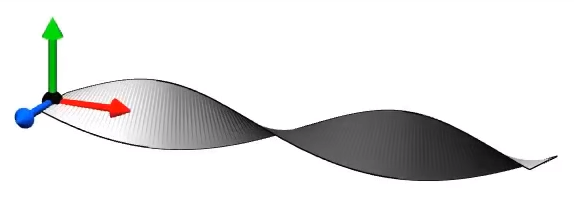
\includegraphics[scale=0.12]{Pictures/xaxisbelt.png} & 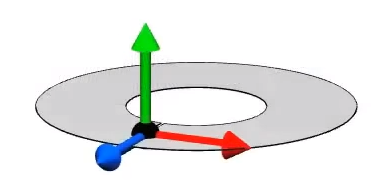
\includegraphics[scale=0.15]{Pictures/yaxisbelt.png} & 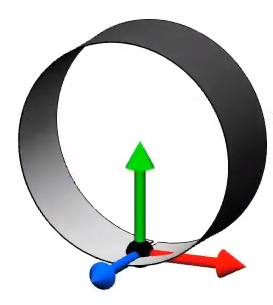
\includegraphics[scale=0.15]{Pictures/zaxisbelt.png} \\
        $\updownarrow$ & $\updownarrow$ & $\updownarrow$ & $\updownarrow$ \\
        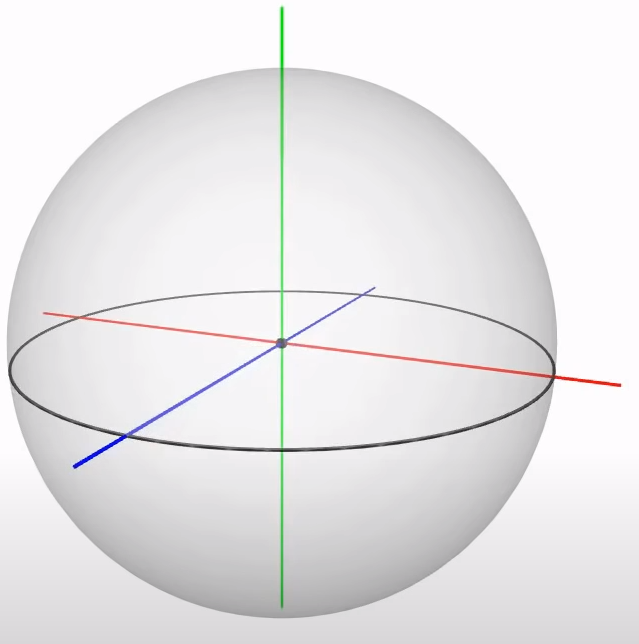
\includegraphics[scale=0.1]{Pictures/4pisphere4.png} & 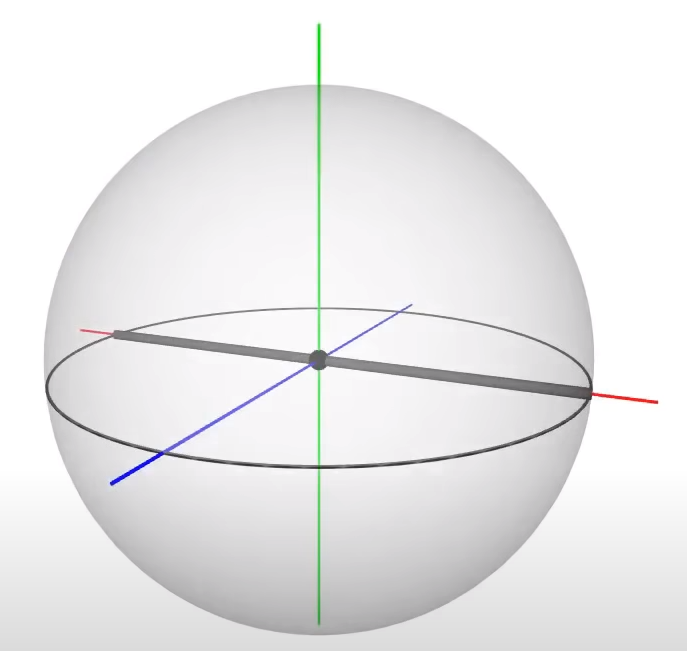
\includegraphics[scale=0.1]{Pictures/xaxissphere.png} & 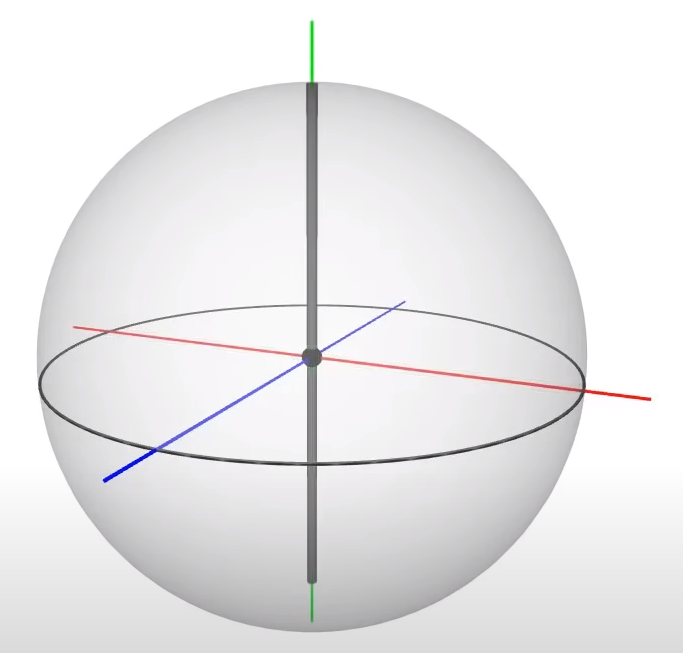
\includegraphics[scale=0.1]{Pictures/yaxissphere.png} & 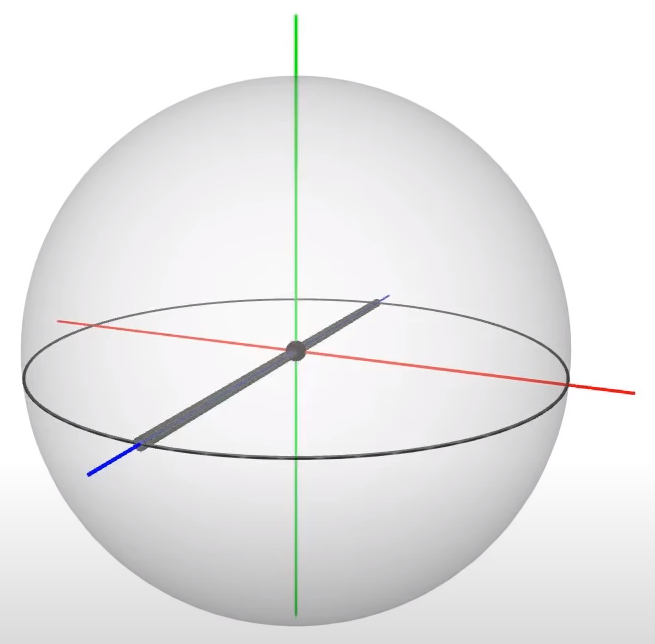
\includegraphics[scale=0.1]{Pictures/zaxissphere.png}
    \end{tabular}}
\end{frame}

\begin{frame}{Dictionary}
    \begin{center}
    \begin{tabular}{ccc}
        \textbf{\underline{random rotation}} & \textbf{\underline{closed}} & \textbf{\underline{open path}}\\
        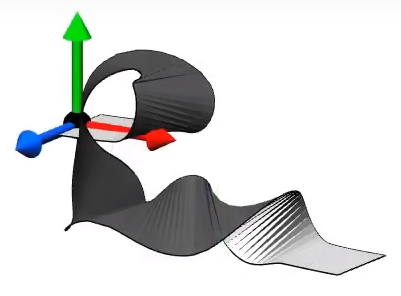
\includegraphics[scale=0.15]{Pictures/randomrotbelt.png} & 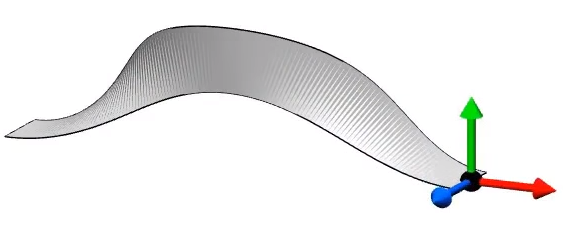
\includegraphics[scale=0.1]{Pictures/contractiblepathbelt.png} & 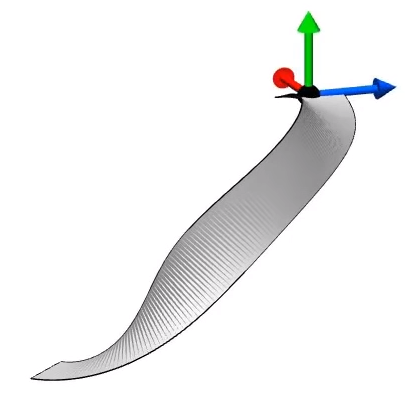
\includegraphics[scale=0.1]{Pictures/noncontractiblepathbelt.png} \\
        $\updownarrow$ & $\updownarrow$ & $\updownarrow$ \\
        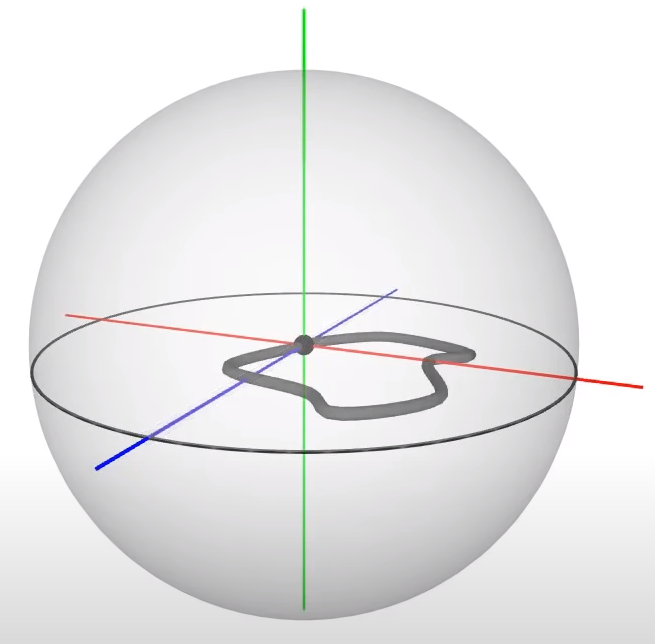
\includegraphics[scale=0.1]{Pictures/randomrotsphere.png} & 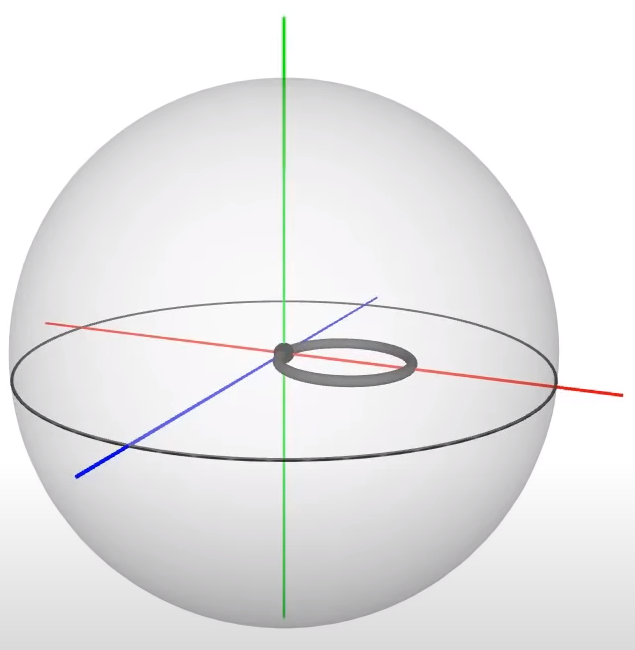
\includegraphics[scale=0.08]{Pictures/contractiblepathsphere.png} & 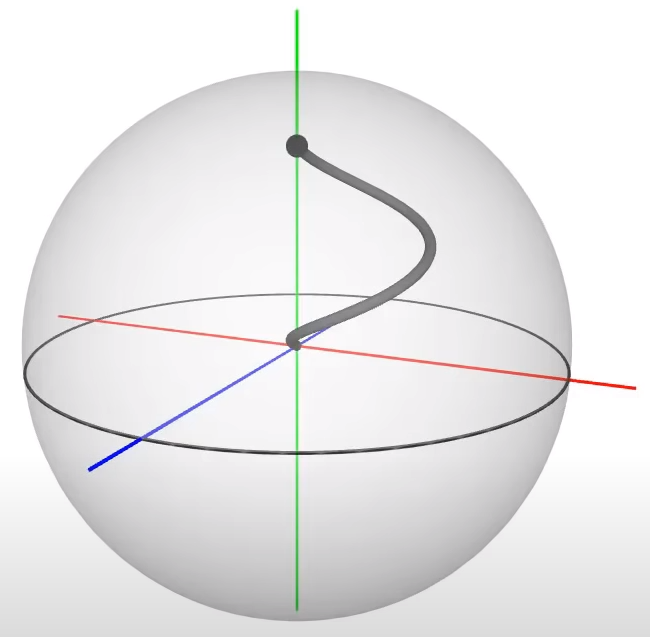
\includegraphics[scale=0.08]{Pictures/noncontractiblepathsphere.png}
    \end{tabular}
    \end{center}
\end{frame}

\begin{frame}{Dictionary}
    \begin{center}
    \begin{tabular}{|ccc|}
        \hline
        \textbf{\underline{Belt}} & & \textbf{\underline{Path}} \\[0.2cm]
        specific configuration & $\longleftrightarrow$ & specific path \\[0.2cm]
        moving the ends & $\longleftrightarrow$ & continuous deformation  \\[0.2cm]
        ends have same orientation & $\longleftrightarrow$ & closed path (loop) \\[0.2cm]
        \emph{can be flattened} & $\longleftrightarrow$ & \emph{contractible} \\ \hline
    \end{tabular}
    \end{center}
    \textbf{Back to Dirac's belt trick:}
    \begin{enumerate}
        \item ends of the belt have same orientation \textcolor{blue}{$\to$ we consider loops} \\
        \hspace{5.8cm} {\tiny \textcolor{blue}{(passing through the origin)}}
        \item moving the ends of the belt \textcolor{blue}{$\to$ continuous deformation} \\
        \item belt in original (flat) position \textcolor{blue}{$\to$ trivial path}
    \end{enumerate}
    The question then becomes: \textbf{which loops are contractible ?}
\end{frame}

\begin{frame}{Problem solved ?}
    \begin{itemize}
        \item \textbf{\underline{$4\pi$-twist:}}
    We saw in the beginning the the $4\pi$-twist can be flattened, how can we see this in terms of paths ?
    \begin{center}
        \begin{tabular}{m{2cm} m{0.5cm} m{2cm} m{0.5cm} m{2cm}}
            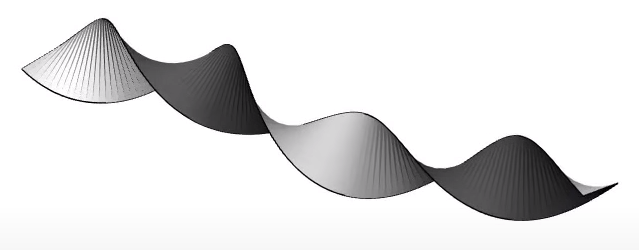
\includegraphics[scale=0.1]{Pictures/4pibelt.png} & $\longleftrightarrow$ & 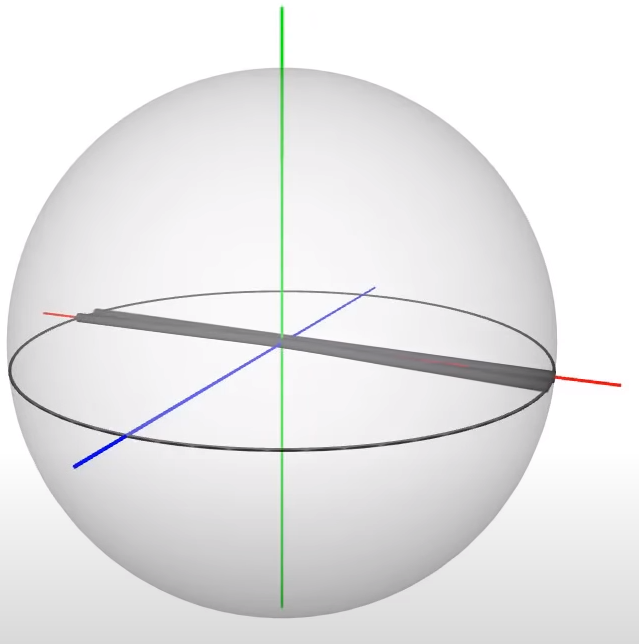
\includegraphics[scale=0.08]{Pictures/4pisphere1.png} & $\longrightarrow$ & 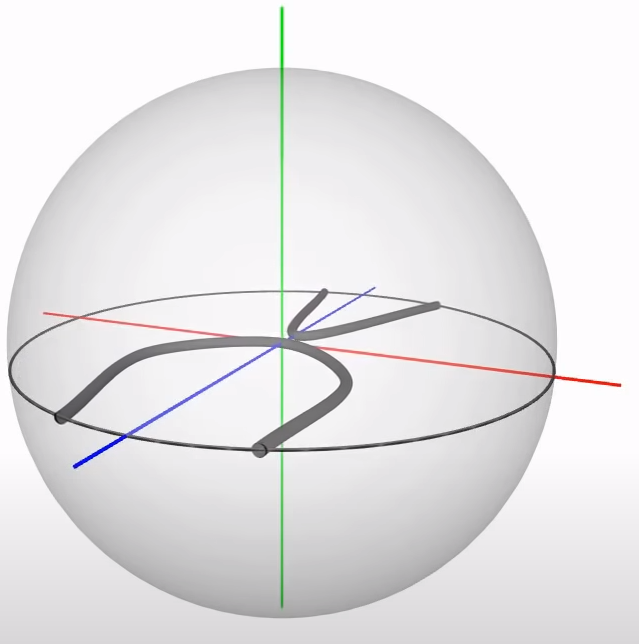
\includegraphics[scale=0.08]{Pictures/4pisphere2.png} \\
            & & & & \hspace{0.7cm} $\downarrow$ \\
            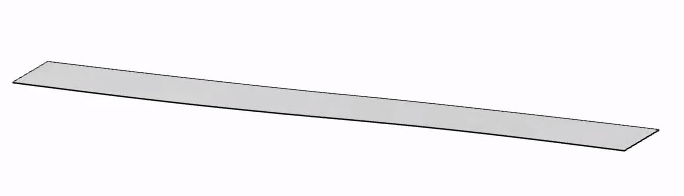
\includegraphics[scale=0.1]{Pictures/flatbelt.png} & $\longleftrightarrow$ & 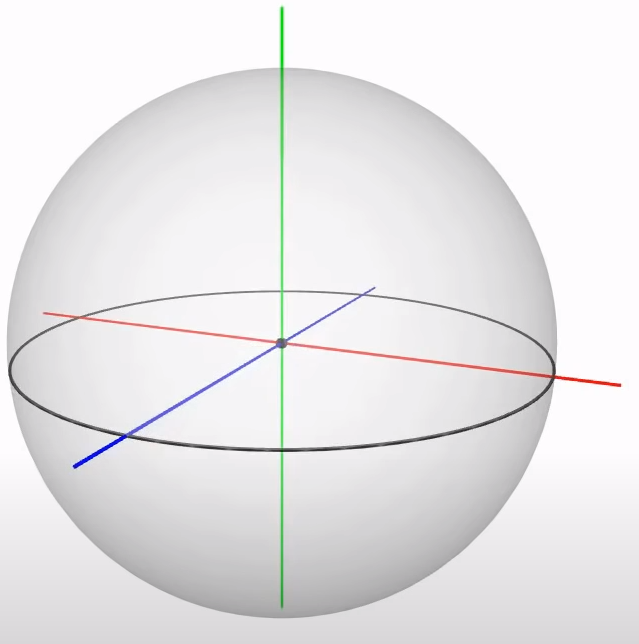
\includegraphics[scale=0.08]{Pictures/4pisphere4.png} & $\longleftarrow$ & 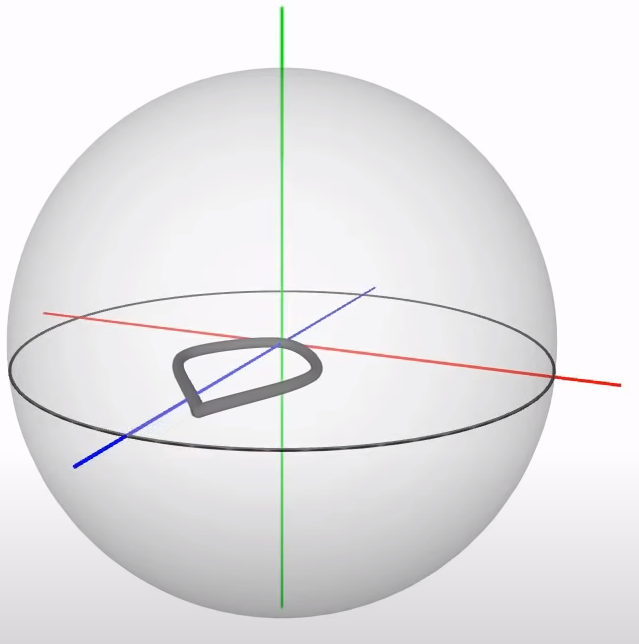
\includegraphics[scale=0.08]{Pictures/4pisphere3.png}
        \end{tabular}
    \end{center}
    $\Rightarrow$ the $4\pi$-twist is \emph{contractible} ! Great.
    \item \textbf{\underline{$2\pi$-twist:}} we ``clearly'' see that is not contractible... no ?! Great..?..  \\[0.2cm]
    \end{itemize}
    \textbf{Wierd aftertaste:} our ``proof'' is good to show contractibility but bad to show non-contractibility and it only works for simple examples.\\
    $\Rightarrow$ We want a consistent and general way of studying paths in topological spaces.
\end{frame}

\section{Homotopy theory}

\begin{frame}{Homotopoy theory primer}
    \textbf{Starting observation:} depending on the topological space, all loops might not be contractible. Moreover, some loops are ``fundamentally different'' from each other.\\
    Examples: $\R^3$, $S^2$, $\mathbb{T}^2$, etc.

    \begin{block}{Paths and homotopies}
        For a topological space $X$:
        \begin{itemize}
            \item \textit{Path} in $X$: continuous map $\gamma:[0,1]\to X$, \textit{loop} if closed
            \item $\gamma_1$ and $\gamma_2$ are \textit{homotopically equivalent} if one can be deformed into the other: there exists
            $H:[0,1]\times [0,1]\to X$ such that
            \begin{equation*}
                H(0,t)=\gamma_1(t)\qquad \text{and}\qquad H(1,t)=\gamma_2(t).
            \end{equation*}
            This is an equivalence relation ($\sim$).
        \end{itemize}
    \end{block}
    
    For each $x_0\in X$, we define
    \begin{equation*}
        \pi_1(X,x_0) = \{\text{all loops based at }x_0\}/\sim,
    \end{equation*}
    it is the set of ``fundamentally different'' loops passing through $x_0$. $[\gamma]$ is called the \textit{homotopy class} of $\gamma$.
\end{frame}

\begin{frame}{Fundamental group}
    Group structure on $\pi_1(X,x_0)$:
    \begin{itemize}
        \item \textbf{Product} of paths: $\gamma_1\cdot\gamma_2=$ ``$\gamma_1$ then $\gamma_2$''
        \item \textbf{Inverse} path: $\gamma^{-1}=$ ``$\gamma$ traversed in the opposite direction''
        \item \textbf{Neutral} path: $e=$ ``constant path at the identity''
        \item For homotopy classes: $[\gamma_1]\cdot[\gamma_2]=[\gamma_1\cdot\gamma_2]$ and $[\gamma]^{-1}=[\gamma^{-1}]$
    \end{itemize}
    Important fact: up to isomorphism, $\pi_1(X,x_0)$ does not depend on $x_0$ \\ $\Rightarrow$ we denote it as $\pi_1(X)$, it is called the \emph{fundamental group} of $X$.\\[0.2cm]
    
    Contractible loops are $\sim$ to a point, i.e. they are the element of $[e]$.\\[0.2cm]

    How to compute $\pi_1(X)$ ? Can be difficult, not discussed here.\\[0.2cm]

    \begin{columns}[T,onlytextwidth]
        \column{0.35\textwidth}
        
            \textbf{Examples:}
            \begin{itemize}
                \item $\pi_1(\R^3)=\{e\}$
                \item $\pi_1(S^2) = \{e\}$
                \item $\pi_1(\mathbb{T}^2)=\textcolor{green}{\Z}\times\textcolor{red}{\Z}$
                \item $\pi_1(\R^2\backslash\{p\})=\Z$
            \end{itemize}
  
        \column{0.65\textwidth}
  
            \begin{figure}
                \centering
                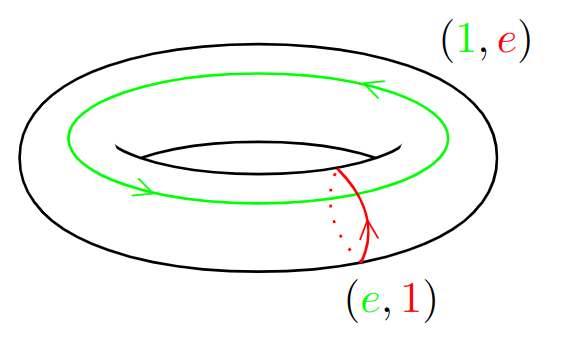
\includegraphics[scale=0.2]{Pictures/torushomotopy3.png}
            \end{figure}
  
    \end{columns}
    Remark: $\pi_1(\R^3\backslash\{p\})=\{e\}$, higher homotopy groups for higher-dimensional holes ?

\end{frame}

\begin{frame}{Back to $\SO(3)$}
    \textbf{Question we had:} are all loops in $\SO(3)$ contractible ?\\
    In homotopy language: is $\pi_1(\SO(3))$ trivial ?\\[0.2cm]
    \textbf{Answer:} \emph{NO}, one can compute that
    \begin{equation*}
        \boxed{\pi_1(\SO(3))=\Z_2}
    \end{equation*}
    $\Rightarrow$ There only two ``fundamentally different'' loops in $\SO(3)$ !\\
    $\Rightarrow$ all non-contractible loops are deformations of the $2\pi$-twist !

    \begin{center}
        \begin{tabular}{|l|}
            \hline
            The belt trick is a way of physically demonstrating that the \\ fundamental group of $\SO(3)$ is $\Z_2$.\\ \hline
        \end{tabular}
    \end{center}

    We can now say, with more confidence, that we understood Dirac's belt trick.\\[0.3cm]

    Are there other manifestation of homotopy in our practical world ?\\[0.3cm]

    Yes: the \emph{spin} ! (you don't need a belt, but you need an electron)\\
    Initially, this trick was a demonstration invented by P. Dirac (1902-1984) to explain the notion of spin to his students.

\end{frame}

{
\setbeamercolor{background canvas}{bg=black!100}
\begin{frame}{Animation 1}
    \begin{center}
        \movie[width=10cm,height=5.5cm,showcontrols,loop]{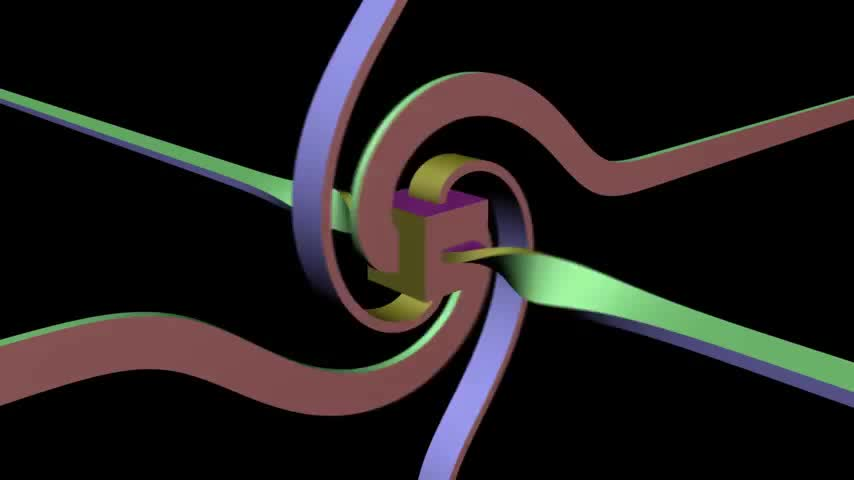
\includegraphics[scale=0.25]{Pictures/poster1.jpg}}{Videos/video1.wmv}
    \end{center}
    {\small\textcolor{white}{An object attached to belts or strings can spin continuously without becoming tangled. Notice that after the cube completes a 360° rotation, the spiral is reversed from its initial configuration. The belts return to their original configuration after spinning a full 720°.}}
\end{frame}

\begin{frame}{Animation 2}
    \begin{center}
        \movie[width=10cm,height=5.5cm,showcontrols,loop]{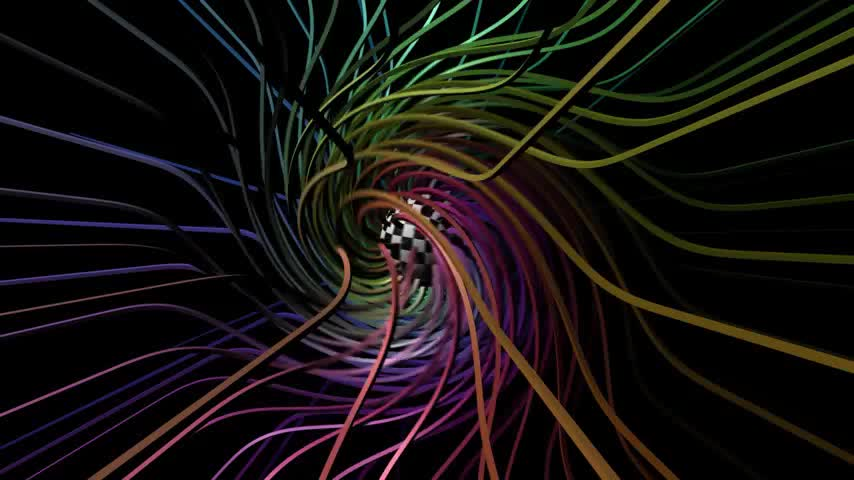
\includegraphics[scale=0.25]{Pictures/poster2.jpg}}{Videos/video2.wmv}
    \end{center}
    {\small\textcolor{white}{A more extreme example demonstrating that this works with any number of strings. In the limit, a piece of solid continuous space can rotate in place like this without tearing or intersecting itself.}}
\end{frame}
}
% https://bloerg.net/posts/beamer-movies-and-linux/

\section{Quantum spin and $\SU(2)$}

\begin{frame}{What is the spin ?}

    Skipping most of the physics background:
    \begin{block}{Spin in quantum mechanics}
        \begin{enumerate}
            \item the \emph{spin}  is an inherent property of any ``particle'':
            \begin{itemize}
                \item number $s\in\frac{1}{2}\N$\textcolor{blue}{, in our case $s=1/2$}
                \item does not change, like the mass, charge, etc
                \item classifies particles
            \end{itemize}
            \item a particle of spin $s$ is, at a given moment, in a certain state described by the \emph{spin vector}:
            \begin{itemize}
                \item unit vector of $v\in\C^{2s+1}$\textcolor{blue}{, in our case $\begin{bmatrix}\alpha\\ \beta\end{bmatrix}\in\C^2$}
                \item can evolve over time
            \end{itemize}
            \item what we can measure yet another quantity, called \emph{observed spin}:
            \begin{itemize}
              \item discrete value $s_{\text{obs.}}\in\{s,s-1,\dots,0,\dots,-s+1,-s\}$\\
              \textcolor{blue}{In our case, $s_{\text{obs.}}\in\{1/2,-1/2\}$ that we denote $\uparrow$ and $\downarrow$}
              \item given a direction, e.g. $i=x,y,z$
              \item outcome is random, we can only compute de probabilities of the different outcomes
            \end{itemize}
        \end{enumerate}
    \end{block}
\end{frame}

\begin{frame}{What is the spin ?}
    \textbf{How do measures happen ?}\\[0.2cm]
    Let us introduce
    {\tiny
    \begin{align*}
        v_{x,\uparrow}=
        \begin{bmatrix}
            1/\sqrt{2} \\ 1/\sqrt{2}
        \end{bmatrix},
        v_{x,\downarrow }=
        \begin{bmatrix}
            1/\sqrt{2} \\ -1/\sqrt{2}
        \end{bmatrix},
        v_{y,\uparrow}=
        \begin{bmatrix}
            1/\sqrt{2} \\ i/\sqrt{2}
        \end{bmatrix},
        v_{y,\downarrow}=
        \begin{bmatrix}
            1/\sqrt{2} \\ -i/\sqrt{2}
        \end{bmatrix},
        v_{z,\uparrow}=
        \begin{bmatrix}
            1 \\ 0
        \end{bmatrix},
        v_{z,\downarrow}=
        \begin{bmatrix}
            0 \\ 1
        \end{bmatrix}.
    \end{align*}}
    The probability of measuring $s_{\text{obs.}}$ in the direction $i$ is given by the projection
    \begin{equation}
        P(i,s_{\text{obs.}}) = \abs{\langle v_{i,k},v \rangle_{\C^2}}^2
    \end{equation}
    where $v$ is the spin vector of the particle.\\[0.2cm]
    \textbf{Example}: in the direction $z$,
    \begin{equation}
      P(z,\uparrow)= \abs{\alpha}^2,\qquad P(z,\downarrow)= \abs{\beta}^2.
    \end{equation}
    Consequently:
    \begin{itemize}
        \item we must have $\langle v,v\rangle_{\C^2}=\abs{\alpha}^2+\abs{\beta}^2=1$
        \item to ``measure'' the spin state, we must repeat the experience many times
        \item there are states that are always spin $\uparrow$ or always spin $\downarrow$
    \end{itemize}
\end{frame}

\begin{frame}{Rotating a spin vector}
    \textbf{\underline{For vectors:}} recall that the scalar product on $\R^3$ is $\langle v_1,v_2\rangle_{\R^3}=(v_1)^Tv_2$ and
    \begin{equation*}
        \langle Rv_1,Rv_2\rangle_{\R^3} = \langle v_1,v_2\rangle_{\R^3}\qquad \Leftrightarrow\qquad R^T R = \mathbbm{1}
    \end{equation*}
    so $\SO(3)$ is the isometry group of $\R^3$ (+ orientation preserving).\\[0.2cm]
    \textbf{\underline{For spin vectors:}} the scalar product on $\C^2$ is $\langle v_1,v_2\rangle_{\C^2}=(v_1)^\dagger v_2$ and
    \begin{equation*}
        \langle Uv_1,Uv_2\rangle_{\C^2} = \langle v_1,v_2\rangle_{\C^2}\qquad \Leftrightarrow\qquad U^\dagger U = \mathbbm{1}
    \end{equation*}
    so, similarly,
    \begin{block}{Special unitary group}
        $\SU(2)$ is the set of $2\times 2$ complex matrices such that $U^\dagger U=\mathbbm{1}$ and $\det U=1$.
    \end{block}
    and $\SU(2)$ is the isometry group of $\C^2$ (+ orientation preserving).\\[0.2cm]
    Like $\SO(3)$ it is a Lie group so it can be viewed
\end{frame}

\begin{frame}{$\SU(2)$ and $\S0(3)$}
    What is the most general for of $U\in\SU(2)$ ? Imposing $U^\dagger=U^{-1}$ and $\det U=1$, we find
    \begin{equation}
        U=
        \begin{bmatrix}
            X+iY & Z+iW \\
            -Z+iY & X-iY
        \end{bmatrix}
    \end{equation}
    with $X^2+Y^2+Z^2+W^2=1$ $\Rightarrow \SU(2)\cong S^3$\\
    so $\SU(2)$ can be viewed as a group and a manifold, it is a Lie group\\[0.2cm]
    $\SU(2)$ and $\SO(3)$:
    \begin{enumerate}
        \item both Lie groups of dimension three
        \item both are connected
        \item $-\mathbbm{1}\in\SU(2)$ but $-\mathbbm{1}\notin\SO(3)$
    \end{enumerate}
    How could we represent $\SU(2)\cong S^3$ in $3d$ ?\\[0.2cm]
    Observation: $S^2$ is equivalent to two disks glued along their boundary\\[0.2cm]
    Similarly: $S^3$ is equivalent to balls glued along their boundary\\[0.2cm]
    \textbf{BUT}, are those spheres related to $\SO(3)$ ?\\
    In other words: how are the two notions of rotations related ?\\[0.2cm]
    $\Rightarrow$ covering spaces !
\end{frame}

\section{Covering spaces}

\begin{frame}{Covering spaces}

    
    \begin{columns}[T,onlytextwidth]
        \column{0.65\textwidth}
        
        \begin{block}{Covering space}
            For a topological space $X$, a \textit{covering space} is a topological space $E$ with a \textit{projection map} $\pi=E\to X$ such that
            \begin{itemize}
                \item $\pi$ is continuous
                \item there exists a discrete set $D$ and $U$ and open neighborhood of $x\in X$ such that
                \begin{equation*}
                    \pi^{-1}(U)=\bigsqcup_{d\in D}V_d
                \end{equation*}
                and $\pi|_{V_d}=V_d\to U$ is a homeomorphism. $V_d$ are called the \textit{sheets}.
            \end{itemize}
        \end{block}
  
        \column{0.35\textwidth}
  
            \begin{figure}
                \centering
                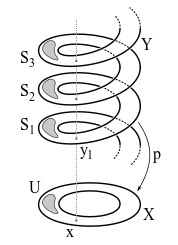
\includegraphics[scale=0.5]{Pictures/Covering_map.png}
            \end{figure}
  
    \end{columns}
    \textbf{Examples:}
    \begin{itemize}
        \item $\R$ can cover $S^1$ with $\pi(t)=(\cos(2\pi t),\sin(2\pi t))$
        \item $S^1$ can cover $S^1$ in several ways, with $\pi(z)=z^n$, $n\in\N$ ($1$ turn in covering space is $n$ turns in $S^1$) 
\includegraphics[scale=0.06]{Pictures/pen.png}
    \end{itemize}

\end{frame}

\begin{frame}{Properties of the coverin space}
    Important remarks:
    \begin{enumerate}
        \item 
    \end{enumerate}
\end{frame}

\begin{frame}
    Proof that $2\pi$-twist is non-contractible in $\SO(3)$
\end{frame}

\section{Spinors}

% take a step back on the first part
% we discussed something for in three dimensions (with SO(3) and SU(2)), how can we generalize this ?
% motivation: any rotation in R^3 can be achived in two topologically inequivalent ways, why should objects be blind to that ? The most general object is spinors
% how to distinguish the topoogically inequivalent rotations ? Universal cover of the group, double cover, spin groups
% properties of the spin groups; in any dimension, actully always TWO topologically inequivalent ways of achiving a rotation, i.e. it is lways a DOUBLE cover, it is unique, maximal, etc
% def of spinor
% other definition of spinor: Clifford algebras, def the algebra
% link with the other definition: Both the spin group and its Lie algebra are embedded inside the Clifford algebra in a natural way, and in applications the Clifford algebra is often the easiest to work with.
% representation theory of the CLifford algebra, i.e. spinors in all dimensions
% come back the three dimensions, our example of SU(2) etc, with representations theory of SO(3) and SU(3), integer spin and half-interger spins

\section{Short detour: spinors in Physics}

% instead of SO(3), SO(1,3), which somewhat resembles SO(4)
% why do we need spinors ? For indistinguishable particles, only two possibilities: fermions and boson
% veri very important theorem relates this and what we discussed: Spin-statistic thm: boson have integer spin and fermions half-integer spin

\section{Conclusion}

\begin{frame}
    \begin{enumerate}
        \item There are two topologically distinguishable classes (homotopy classes) of paths through rotations that result in the same overall rotation, as illustrated by the Dirac's belt trick. (True in any dimension)
        \item Spinors change in different ways depending not just on the overall final rotation, but the details of how that rotation was achieved (by a continuous path in the rotation group).
        \item The spin group is the group of all rotations keeping track of the class. It doubly covers the rotation group, since each rotation can be obtained in two inequivalent ways as the endpoint of a path.
        \item The space of spinors by definition is equipped with a (complex) linear representation of the spin group.
    \end{enumerate}
\end{frame}

\begin{frame}{Blocks}
    Three different block environments are pre-defined and may be styled with an
    optional background color.
  
    \begin{columns}[T,onlytextwidth]
        \column{0.5\textwidth}
          
            Some text.\\[2cm]
            aaaaa
    
        \column{0.5\textwidth}
    
            \begin{block}{Default}
              Block content.
            \end{block}
      
            \begin{alertblock}{Alert}
              Block content.
            \end{alertblock}
      
            \begin{exampleblock}{Example}
              Block content.
            \end{exampleblock}
    
    \end{columns}

\end{frame}

\appendix

{
\setbeamercolor{background canvas}{bg=green!10}

\begin{frame}{Introduction to the spin}
    
    \begin{block}{Spin in quantum mechanics}
        The \emph{spin} of an ``particle'' is a number $s\in\frac{1}{2}\N$.\\
        The \emph{spin state} of a particle of spin $s$ is a unit vector in $\C^{2s+1}$.
    \end{block}
    The spin is a \emph{property}, it cannot change (e.g. mass, charge)\\
    The spin state is a \emph{characteristic}, it evolves

    How to interpret it ? 
    \begin{enumerate}
        \item \textbf{directions:} we choose the direction in which we want to measure it
        \item \textbf{probabilistic theory:} the outcome of the measure, we can only compute the probabilities of the different outcomes
        \item \textbf{discrete quantity:} in the chosen direction, the spin will either appear to up or down ($\uparrow$ or $\downarrow$)
    \end{enumerate}
    The probability of measuring the spin $k=\uparrow,\downarrow$ in the direction $i=x,y,z$ is given by
    \begin{equation}
        P(i,k) = \abs{\langle v_{i,k},v \rangle}^2
    \end{equation}
    where $v$ is the spin state of the particle, for some given vectors $v_{i,k}$.

\end{frame}

\begin{frame}{Spin in quantum mechanics}
    The Lie algebra $\mathfrak{su}(2)$ is generated by the \emph{Pauli matrices}
    \begin{equation}
        \sigma_x =
        \begin{bmatrix}
            0 & 1\\
            1 & 0
        \end{bmatrix},\qquad
        \sigma_y =
        \begin{bmatrix}
            0 & -i\\
            i & 0
        \end{bmatrix},\qquad
        \sigma_z =
        \begin{bmatrix}
            1 & 0\\
            0 & -1
        \end{bmatrix}.
    \end{equation}
    
\end{frame}

}

\begin{frame}[allowframebreaks]{References}

\bibliography{bibliography}
\bibliographystyle{abbrv}

\end{frame}

\end{document}
